\documentclass[12pt,a4paper]{article}

% --- Essential Packages ---
\usepackage[a4paper, top=0.85in, bottom=0.90in, left=1in, right=1in, headheight=15pt, footskip=0.42in]{geometry}
\usepackage{mathptmx}      % Times Roman typography
\usepackage{inconsolata}   % Razor-sharp, proportional programming font
\usepackage{upquote}       % Straight single quotes for code strings
\usepackage{graphicx}
\usepackage{listings}
\usepackage{array}
\usepackage{booktabs}
\usepackage{tabularx}
\usepackage{fancyhdr}
\usepackage{titlesec}
\usepackage{setspace}
\usepackage{enumitem}
\usepackage{refcount}
\usepackage{hyperref}

% --- Line Spacing & Paragraph Layout ---
\setstretch{1.18}
\setlength{\parskip}{0.4em}
\setlength{\parindent}{0pt}

% --- Strict Anti-Orphan, Anti-Widow & Flush Control ---
\widowpenalty=10000
\clubpenalty=10000
\brokenpenalty=10000
\raggedbottom

% --- Compact List Spacing (Rule 2) ---
\setlist[itemize]{noitemsep, topsep=2pt, parsep=1pt, partopsep=0pt, leftmargin=1.5em}
\setlist[enumerate]{noitemsep, topsep=2pt, parsep=1pt, partopsep=0pt, leftmargin=1.5em}

% --- Pure Black & White Hyperlinks ---
\hypersetup{
    colorlinks=false,
    pdfborder={0 0 0}
}

% --- Header & Footer Configuration ---
\pagestyle{fancy}
\fancyhf{}
\fancyfoot[R]{\textit{Bank Management System \quad$|$\quad Page \thepage}}
\renewcommand{\headrulewidth}{0pt}
\renewcommand{\footrulewidth}{0.5pt}

% --- High-Impact Heading Formatting (Pure B&W) ---
\titleformat{\section}
  {\normalfont\Huge\bfseries\centering}
  {}{0em}
  {\MakeUppercase}
  [\vspace{0.4ex}\rule{\textwidth}{1.6pt}]

\titleformat{\subsection}
  {\normalfont\Large\bfseries}
  {}{0em}
  {\MakeUppercase}
  [\vspace{0.2ex}\rule{\linewidth}{0.6pt}]

\titleformat{\subsubsection}
  {\normalfont\large\bfseries}
  {}{0em}
  {}

\titlespacing*{\section}{0pt}{4pt}{8pt}
\titlespacing*{\subsection}{0pt}{8pt}{4pt}
\titlespacing*{\subsubsection}{0pt}{6pt}{3pt}

% --- Distortion-Free Listings Configuration for Python Code ---
\lstset{
    basicstyle=\fontsize{9pt}{11.2pt}\selectfont\ttfamily,
    columns=flexible,
    keepspaces=true,
    showstringspaces=false,
    breaklines=true,
    breakatwhitespace=true,
    breakindent=10pt,
    frame=single,
    framerule=0.7pt,
    framesep=5pt,
    xleftmargin=6pt,
    xrightmargin=6pt,
    tabsize=4,
    aboveskip=6pt,
    belowskip=6pt,
    keywordstyle=\bfseries,
    commentstyle=\itshape,
    stringstyle=\normalfont\ttfamily
}

% --- Dynamic Two-Digit Page Reference Macro for Index ---
\newcommand{\pnum}[2]{%
  \ifnum\getpagerefnumber{#1}>0\relax
    \hyperlink{#1}{\ifnum\getpagerefnumber{#1}<10 0\fi\pageref*{#1}}%
  \else
    \hyperlink{#1}{#2}%
  \fi
}

\begin{document}

% =========================================================================
% PAGE 3: INDEX
% =========================================================================
\setcounter{page}{3}

\section*{INDEX}
\vspace{1.5em}

\begin{center}
\renewcommand{\arraystretch}{1.38}
\begin{tabular}{|c|p{10.5cm}|c|}
\hline
\textbf{SER} & \textbf{DESCRIPTION} & \textbf{PAGE NO} \\ \hline
01 & INTRODUCTION & \pnum{sec:intro}{04} \\ \hline
02 & OBJECTIVES OF THE PROJECT & \pnum{sec:objectives}{05} \\ \hline
03 & PROPOSED SYSTEM & \pnum{sec:proposed}{06} \\ \hline
04 & SYSTEM DEVELOPMENT LIFE CYCLE (SDLC) & \pnum{sec:sdlc}{07} \\ \hline
05 & PHASES OF SYSTEM DEVELOPMENT LIFE CYCLE & \pnum{sec:phases}{08} \\ \hline
06 & FLOW CHART & \pnum{sec:flowchart}{15} \\ \hline
07 & SOURCE CODE & \pnum{sec:sourcecode}{17} \\ \hline
08 & OUTPUT & \pnum{sec:output}{23} \\ \hline
09 & TESTING & \pnum{sec:testing}{29} \\ \hline
10 & HARDWARE AND SOFTWARE REQUIREMENTS & \pnum{sec:hardware}{32} \\ \hline
11 & INSTALLATION PROCEDURE & \pnum{sec:installation}{33} \\ \hline
12 & BIBLIOGRAPHY & \pnum{sec:bibliography}{34} \\ \hline
\end{tabular}
\end{center}

\vfill
\begin{center}
\small\textit{Note: The Acknowledgement section is independently maintained for submission.}
\end{center}

\clearpage

% =========================================================================
% PAGE 4: INTRODUCTION
% =========================================================================
\phantomsection\hypertarget{sec:intro}{}\label{sec:intro}
\section*{01. INTRODUCTION}
\vspace{0.5em}

In the contemporary financial landscape, the modernization and digitization of commercial operations have transitioned from an operational convenience to an imperative necessity. The \textbf{``BANK MANAGEMENT SYSTEM''} is a dedicated database-backed software application engineered to handle, automate, and streamline everyday branch-level accounting and administrative responsibilities.

\vspace{0.4em}
For decades, financial establishments operated via manual physical ledgers, ink-and-paper journals, and paper registers. While traditionally functional, these legacy mechanisms suffer from severe limitations: human calculation fatigue, mathematical discrepancies, catastrophic physical vulnerability to fire or water, and extreme labor delays during routine account reconciliations. Locating a single historical transaction often demanded digging through hundreds of archived binders.

\vspace{0.4em}
The emerging paradigm of digital information systems makes comprehensive customer and transaction intelligence accessible instantaneously. By deploying a computerized architecture, customer account opening, verification, deposits, withdrawals, and ledger adjustments are completed within fractions of a second.

\vspace{0.4em}
\subsection*{Core Pillars of the System}
\begin{itemize}
    \item \textbf{Operational Efficiency:} Eliminating customer queue congestion by enabling high-speed automated credit and debit operations directly at the teller console.
    \item \textbf{Data Security \& User Access Control:} Restricting system access to authorized operators through unique operator IDs and mandatory 4-digit PIN authentication.
    \item \textbf{Referential Integrity:} Synchronizing customer profiles with append-only transaction audit logs to guarantee that every financial debit or credit is permanently logged with an automated date timestamp.
    \item \textbf{Real-Time Reporting:} Providing immediate terminal reports on customer account balances and full historical account statements without manual calculation.
\end{itemize}

\vspace{0.4em}
Developed utilizing \textbf{Python 3.12} and \textbf{MySQL Database Management System}, this project exemplifies the application of core computer science fundamentals to an authentic commercial requirement, serving as an extensible prototype for computerized financial administration.

\clearpage

% =========================================================================
% PAGE 5: OBJECTIVES OF THE PROJECT
% =========================================================================
\phantomsection\hypertarget{sec:objectives}{}\label{sec:objectives}
\enlargethispage{\baselineskip}
\section*{02. OBJECTIVES OF THE PROJECT}
\vspace{0.5em}

The fundamental objective of this project is to bridge theoretical computer science pedagogy with real-world software engineering, equipping students with practical software design, database interfacing, and system validation skills.

\vspace{0.4em}
\subsection*{1. Technical Objectives}
\begin{itemize}
    \item \textbf{Relational Database Architecture:} Design and implement a normalized database schema in MySQL comprising distinct entity tables (\texttt{user\_table}, \texttt{customer\_details}, and \texttt{transactions}) with primary key and foreign key relationships.
    \item \textbf{Python-MySQL Connectivity:} Establish reliable client-server communication using Python's standard \texttt{mysql.connector} library to execute dynamic Data Definition (DDL) and Data Manipulation (DML) queries.
    \item \textbf{Clean Procedural Programming:} Construct modular, maintainable, and readable procedural code strictly conforming to the CBSE Class 12 Computer Science syllabus, utilizing clean functions and standard library modules like \texttt{datetime}.
    \item \textbf{Overdraft \& Fraud Prevention:} Implement rigorous programmatic validation checks to prevent negative account balances by rejecting withdrawal requests exceeding existing credit reserves.
\end{itemize}

\vspace{0.4em}
\subsection*{2. Operational Objectives}
\begin{itemize}
    \item \textbf{Automated Profile Management:} Automate new customer onboarding, account number assignment, and residential detail cataloging.
    \item \textbf{Atomic Transaction Logging:} Guarantee ACID (Atomicity, Consistency, Isolation, Durability) principles by issuing explicit database commit directives (\texttt{conn.commit()}) following every balance modification.
    \item \textbf{Complete Auditability:} Maintain an indelible, chronological transaction register detailing the transaction date, account identifier, withdrawal sum, and deposited sum for auditing purposes.
\end{itemize}

\vspace{0.4em}
\subsection*{3. Academic \& Methodological Goals}
\begin{itemize}
    \item To demonstrate comprehensive grasp of the \textbf{Software Development Life Cycle (SDLC)} across initiation, concept analysis, structured design, coding, and empirical testing.
    \item To develop practical expertise in writing technical software documentation, designing formal ANSI flowcharts, modeling Entity-Relationship (ER) diagrams, and executing structured test cases.
\end{itemize}

\clearpage

% =========================================================================
% PAGE 6: PROPOSED SYSTEM
% =========================================================================
\phantomsection\hypertarget{sec:proposed}{}\label{sec:proposed}
\section*{03. PROPOSED SYSTEM}
\vspace{0.4em}

\subsection*{Shortcomings of the Existing Manual System}
Under traditional manual banking workflows, all customer transactions are transcribed into physical paper ledgers. This archaic operational model exhibits multiple critical points of failure:
\begin{itemize}
    \item \textbf{Human Calculation Inaccuracies:} Tellers calculating balances manually during peak business hours frequently introduce arithmetic errors that compromise institutional accounts.
    \item \textbf{Data Redundancy \& Duplication:} Customer profiles must be transcribed across multiple register books, causing data drift and inconsistency.
    \item \textbf{Sluggish Query Retrieval:} Auditing a customer's balance or past statements requires laborious manual searching through historical ledgers.
    \item \textbf{Vulnerability to Destruction:} Physical registers degrade over time and are completely defenseless against termites, dampness, fire hazards, and theft.
\end{itemize}

\subsection*{Architecture \& Capabilities of the Proposed System}
The proposed computerized \textbf{Bank Management System} introduces an integrated digital environment that overcomes every manual bottleneck. Written in Python 3.12, the application interfaces with a high-performance local MySQL relational database engine. All transaction arithmetic is automated by the processor, completely eliminating human mathematical error. Account updates, profile lookups, and transaction logging happen synchronously in milliseconds.

The application's operational flow is organized around distinct, self-contained modules --- authentication, account administration, transaction processing, and reporting --- each rigorously isolated to prevent cascading failures. Every operator interaction is routed through a unified, menu-driven console that mirrors real-world teller workflows, so non-technical staff can adopt the system with minimal training. The architecture deliberately favors transparent, data-centric operations over complex abstractions, ensuring that each screen transition maps directly to a verifiable database action.

\vspace{0.4em}
\begin{figure}[H]
    \centering
    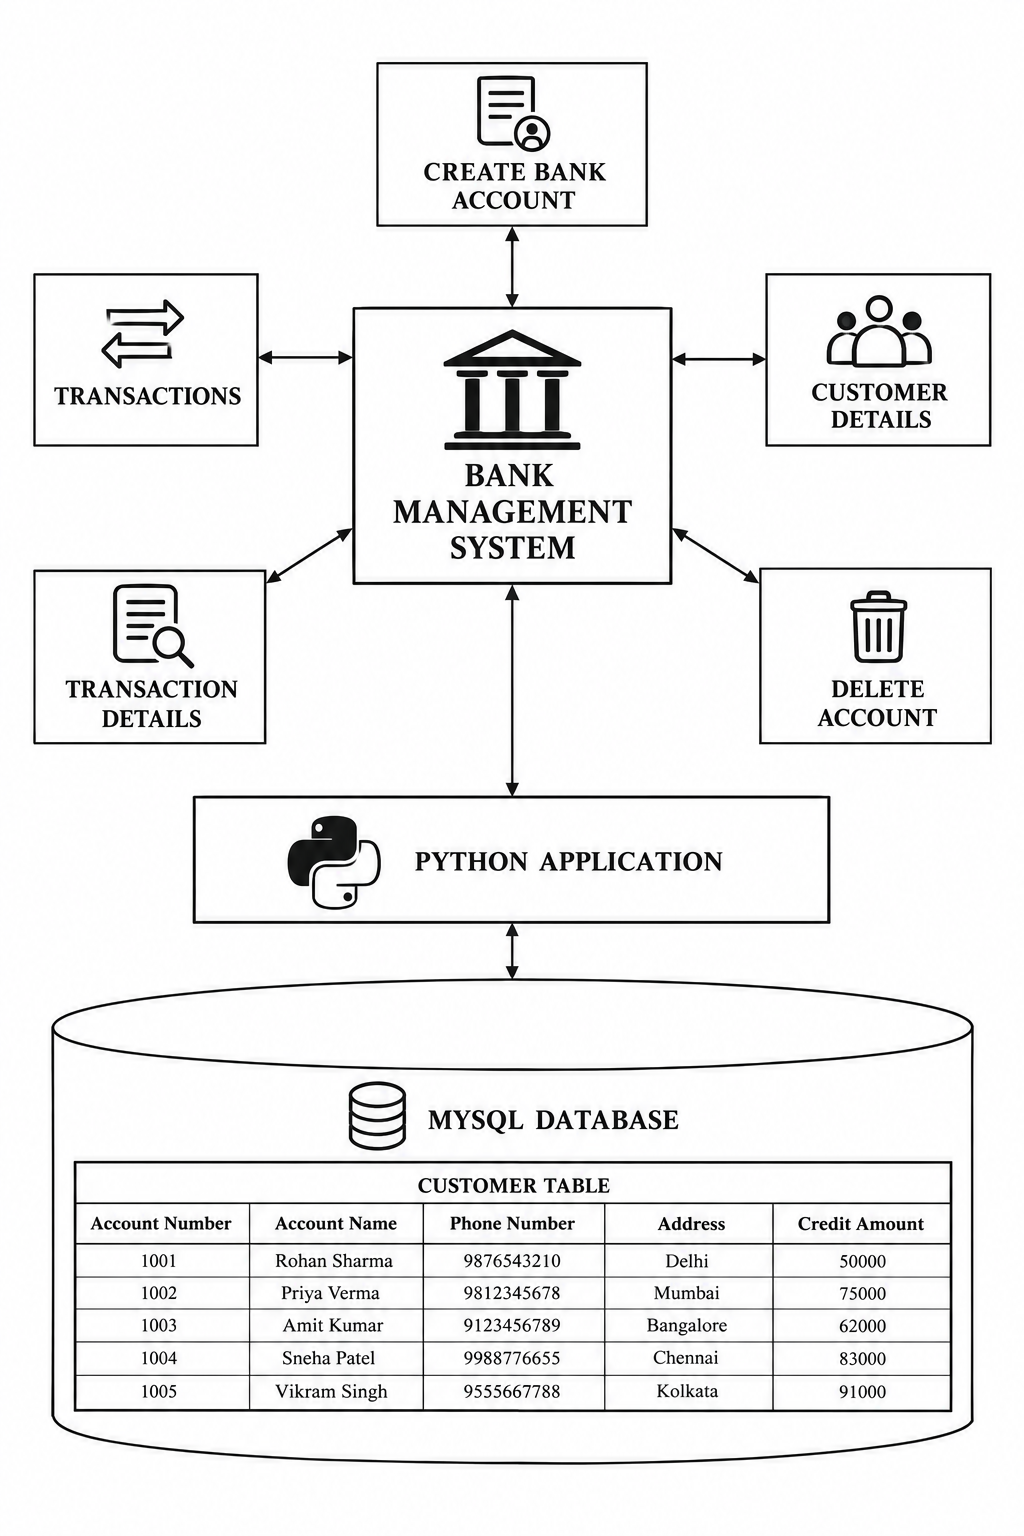
\includegraphics[width=0.62\textwidth]{images/1.png}
    \caption{\textit{Bank Management System Architecture Diagram}}
\end{figure}

\clearpage

% =========================================================================
% PAGE 7: SYSTEM DEVELOPMENT LIFE CYCLE (SDLC)
% =========================================================================
\phantomsection\hypertarget{sec:sdlc}{}\label{sec:sdlc}
\section*{04. SYSTEM DEVELOPMENT LIFE CYCLE (SDLC)}
\vspace{0.5em}

The Systems Development Life Cycle (SDLC) is a foundational project management framework that divides complex software engineering projects into distinct, manageable, and verifiable phases. Implementing a formal SDLC methodology ensures that engineering risks are diagnosed early, requirements are validated comprehensively, and software artifacts undergo quality assurance before deployment.

\vspace{0.4em}
In financial software development, where data integrity and transaction accuracy are mission-critical, adhering to an established SDLC process protects the system against design flaws, unhandled exceptions, and data corruption. The iterative lifecycle followed during this project is diagrammed below:

\vspace{0.6em}
\begin{figure}[H]
    \centering
    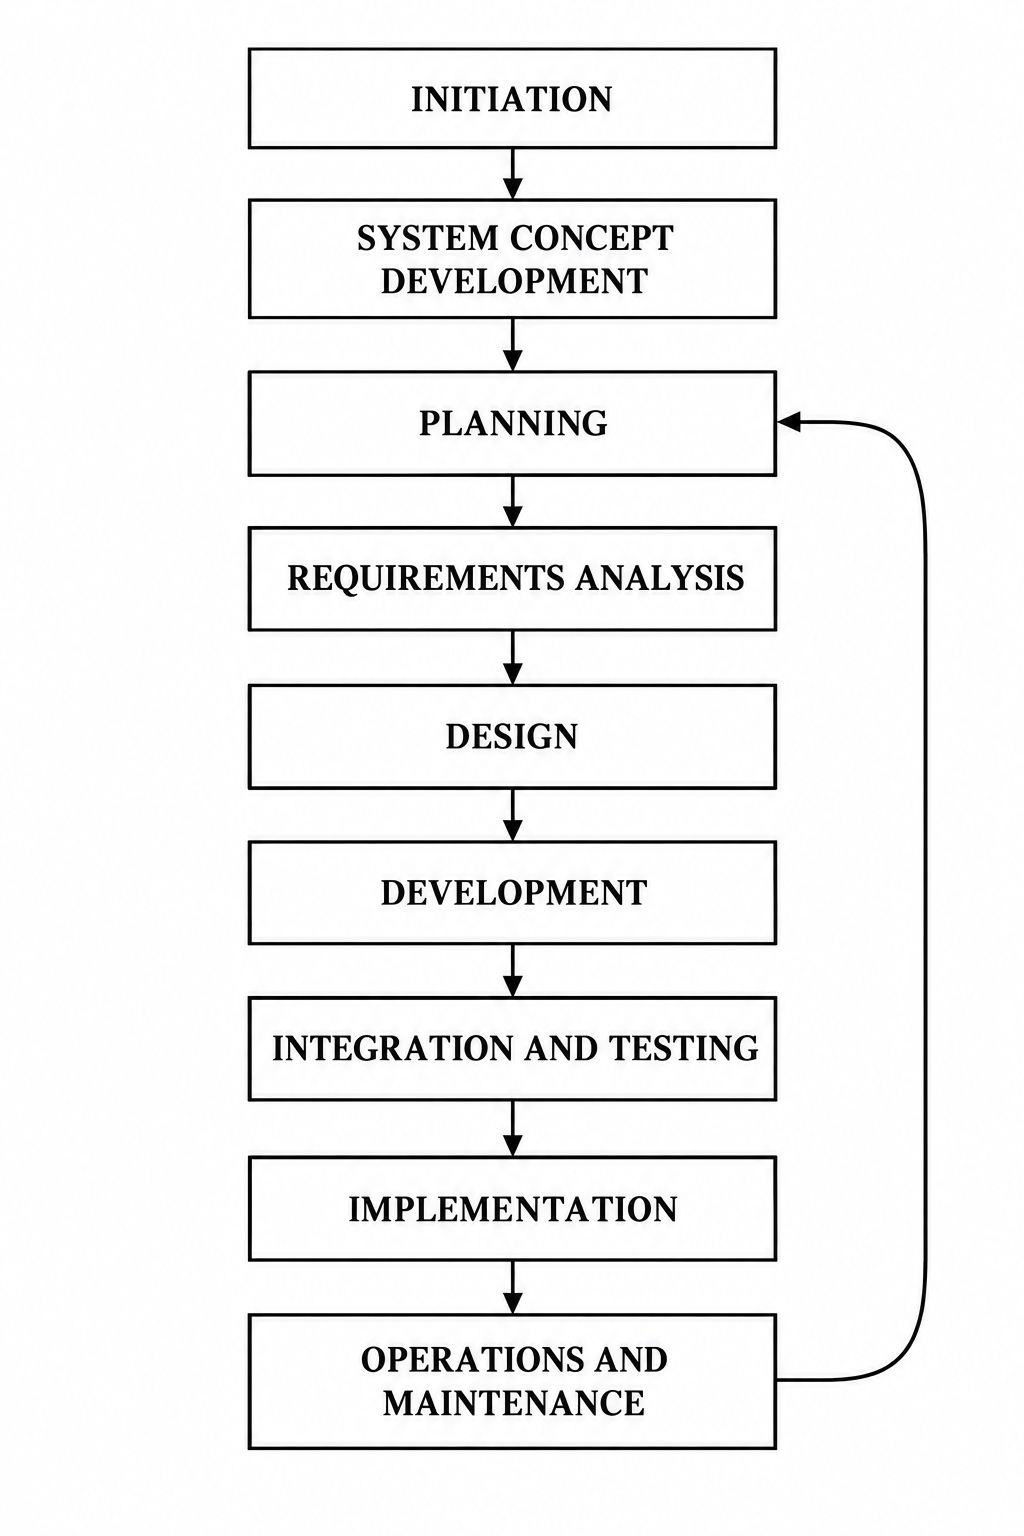
\includegraphics[width=0.46\textwidth]{images/2.png}
    \caption{\textit{Software Development Life Cycle (SDLC) Flowchart}}
\end{figure}

\clearpage

% =========================================================================
% PAGE 8: PHASES OF SDLC (Phase 1 & Phase 2)
% =========================================================================
\phantomsection\hypertarget{sec:phases}{}\label{sec:phases}
\section*{05. PHASES OF SYSTEM DEVELOPMENT LIFE CYCLE}
\vspace{0.5em}

\subsection*{PHASE 1: INITIATION PHASE}
The Initiation Phase marks the genesis of the project. It establishes whether an automated software system is justified to replace manual banking registers and defines the project's strategic and operational boundaries.

\vspace{0.4em}
\noindent\textbf{Key Objectives Accomplished:}
\begin{itemize}
    \item \textbf{Problem Formulation:} Identifying systemic bottlenecks in manual banking operations, specifically ledger calculation errors and account lookup delays.
    \item \textbf{Technical Feasibility Assessment:} Confirming that the combination of Python 3.12 and MySQL provides a stable, zero-license-cost, highly responsive environment for branch-level banking operations.
    \item \textbf{Scope Definition:} Restricting initial software boundaries to user authentication, customer profile cataloging, deposit/withdrawal financial processing, and account inquiries.
    \item \textbf{Stakeholder Alignment:} Establishing project milestones and review cadences under academic guidance.
\end{itemize}

\vspace{1.2em}
\subsection*{PHASE 2: SYSTEM CONCEPT DEVELOPMENT PHASE}
During this phase, the project concept is refined into a concrete operational model. System boundaries, operational interactions, and user classes are analyzed and documented.

\vspace{0.4em}
\noindent\textbf{Key Activities Performed:}
\begin{itemize}
    \item \textbf{System Boundary Demarcation:} Defining the application boundary as a terminal-based console communicating via SQL protocol with a local database daemon.
    \item \textbf{User Persona Identification:} Identifying system operators as authorized branch tellers executing operations on behalf of registered customer accounts.
    \item \textbf{Risk Identification \& Mitigation:} Formulating mitigation strategies for financial edge cases, specifically overdraft withdrawals and SQL injection vulnerabilities.
    \item \textbf{Performance Standards:} Mandating response latencies under 0.5 seconds for routine ledger updates and profile searches.
\end{itemize}

\clearpage

% =========================================================================
% PAGE 9: PHASES OF SDLC (Phase 3 & Phase 4)
% =========================================================================
\subsection*{PHASE 3: PLANNING PHASE}
The Planning Phase translates the project concept into a structured work breakdown schedule. Resource requirements, development milestones, and testing procedures are established to ensure methodical execution.

\vspace{0.4em}
\noindent\textbf{Key Deliverables of this Phase:}
\begin{itemize}
    \item \textbf{Milestone Schedule:} Setting distinct target dates for schema design, script authoring, test case execution, and technical report drafting.
    \item \textbf{Environment Blueprinting:} Documenting runtime software dependencies (Python 3.12 interpreter, MySQL Server 8.0, and the \texttt{mysql-connector-python} package).
    \item \textbf{Quality Assurance Strategy:} Formulating validation standards for user input (4-digit numeric PINs, non-negative transaction amounts, valid 10-digit telephone records).
\end{itemize}

\vspace{1.2em}
\subsection*{PHASE 4: REQUIREMENTS ANALYSIS PHASE}
Requirements Analysis systematically documents the functional and non-functional requirements the software must satisfy.

\vspace{0.4em}
\noindent\textbf{1. Functional Requirements:}
\begin{itemize}
    \item \textbf{Authentication:} Operators must supply a valid username and 4-digit security PIN before gaining dashboard access.
    \item \textbf{Account Registration:} The system must collect and store unique account numbers, account holder legal names, contact numbers, residential locations, and opening deposits.
    \item \textbf{Deposit Processing:} The system must credit specified sums to active accounts and write an audit record to the transaction database.
    \item \textbf{Withdrawal Processing:} The system must verify balance sufficiency, debit approved sums, and write an audit record.
    \item \textbf{Inquiry Functions:} The system must generate instant profile overviews and chronological statement audit logs.
\end{itemize}

\vspace{0.4em}
\noindent\textbf{2. Non-Functional Requirements:}
\begin{itemize}
    \item \textbf{Data Integrity:} Strict preservation of ACID transactional properties across all database write actions.
    \item \textbf{Interface Usability:} An uncluttered, numbered command-line menu providing explicit success and failure feedback.
\end{itemize}

\clearpage

% =========================================================================
% PAGE 10: PHASES OF SDLC (Phase 5: Design)
% =========================================================================
\subsection*{PHASE 5: SYSTEM DESIGN PHASE}
The System Design Phase translates documented requirements into technical blueprints, establishing the structural architecture, modular decomposition, and database specifications.

\vspace{0.6em}
\noindent\textbf{1. Modular Decomposition:}
\begin{itemize}
    \item \textbf{Authentication Gateway (\texttt{main\_bank.py}):} Serves as the security boundary, orchestrating user registration, credential verification, and menu dispatch.
    \item \textbf{Operations Engine (\texttt{menu.py}):} Implements the interactive banking dashboard providing account creation, transactions, inquiries, and termination.
    \item \textbf{Schema Initialization Modules (\texttt{table.py}, \texttt{user\_table.py}, \texttt{transaction\_table.py}):} Automated DDL scripts establishing database tables and constraint rules.
\end{itemize}

\vspace{0.6em}
\noindent\textbf{2. Procedural Control Flow:}
The execution model adheres to an interactive procedural loop. Upon script invocation, the operator authenticates against \texttt{user\_table}. Upon authorization, control passes to \texttt{main\_menu()}, executing a persistent \texttt{while True} operational loop. The loop dispatches user choices (1 through 6) to corresponding database routines and terminates gracefully upon selecting Option 6 (Quit).

\vspace{0.6em}
\noindent\textbf{3. Defensive Validation Logic:}
\begin{itemize}
    \item \textbf{Account Verification:} Validating that an account exists in \texttt{customer\_details} prior to processing any transaction or lookup.
    \item \textbf{Overdraft Protection:} Comparing requested withdrawal amounts against the current balance (\texttt{amt > current\_bal}) before executing SQL updates.
\end{itemize}

\vspace{0.4em}
\begin{figure}[H]
    \centering
    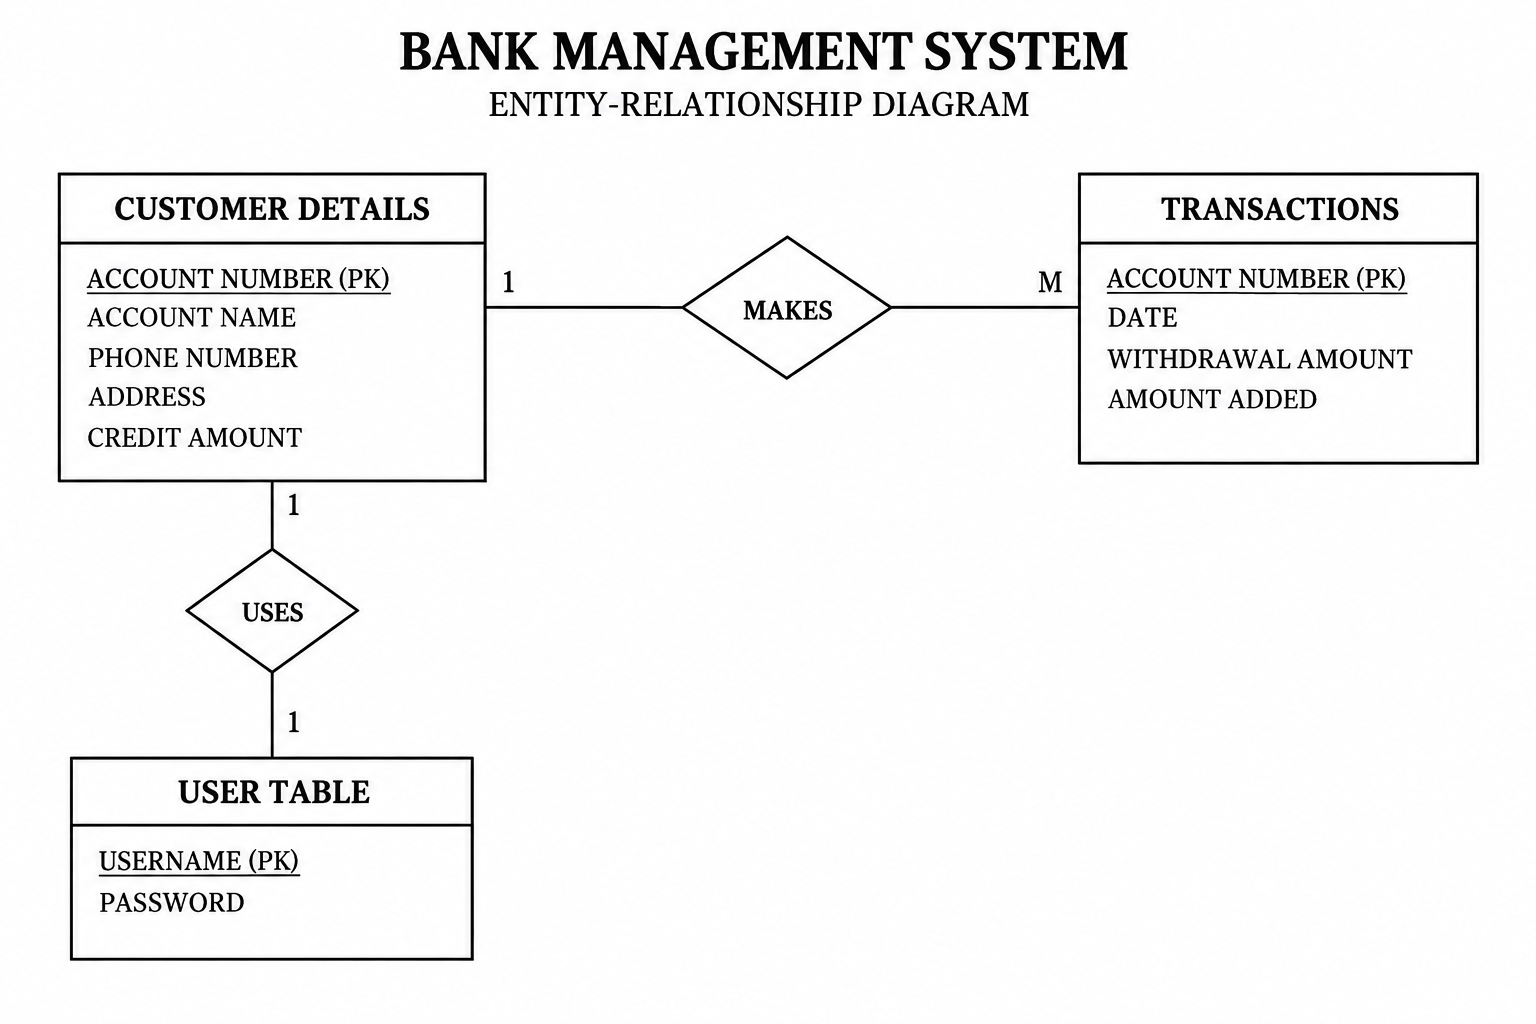
\includegraphics[width=0.55\textwidth]{images/4.png}
    \caption{\textit{Bank Management System Entity-Relationship (ER) Diagram}}
\end{figure}

\clearpage

% =========================================================================
% PAGE 11: PHASES OF SDLC (Database Design & ER Diagram)
% =========================================================================
\subsection*{DATABASE DESIGN \& ENTITY-RELATIONSHIP (ER) MODELING}
Data persistence is managed via a normalized relational database titled \texttt{bank} hosted on MySQL. The schema is organized into three specialized tables:

\vspace{0.4em}
\noindent\textbf{Table 1: \texttt{user\_table} --- Operator Security Credentials}
\begin{itemize}
    \item \texttt{username VARCHAR(25) PRIMARY KEY} --- Unique identifier for system operator.
    \item \texttt{passwrd VARCHAR(25) NOT NULL} --- 4-digit security PIN.
\end{itemize}

\noindent\textbf{Table 2: \texttt{customer\_details} --- Customer Accounts Ledger}
\begin{itemize}
    \item \texttt{acct\_no INT PRIMARY KEY} --- Unique primary key identifying the bank account.
    \item \texttt{acct\_name VARCHAR(25)} --- Full legal name of the account holder.
    \item \texttt{phone\_no BIGINT} --- Customer primary contact phone number.
    \item \texttt{address VARCHAR(50)} --- Residential town or city.
    \item \texttt{cr\_amt FLOAT} --- Current ledger credit balance.
\end{itemize}

\noindent\textbf{Table 3: \texttt{transactions} --- Transaction Audit Trail}
\begin{itemize}
    \item \texttt{acct\_no INT} --- Account identifier linked to \texttt{customer\_details} (Foreign Key).
    \item \texttt{date DATE} --- Chronological date of transaction execution.
    \item \texttt{withdrawal\_amt FLOAT} --- Debited amount (0.0 if deposit).
    \item \texttt{amount\_added FLOAT} --- Credited amount (0.0 if withdrawal).
\end{itemize}

\clearpage

% =========================================================================
% PAGE 12: PHASES OF SDLC (Phase 6: Development)
% =========================================================================
\subsection*{PHASE 6: SOFTWARE DEVELOPMENT PHASE (CODING)}
The Development Phase transforms architectural designs into clean, maintainable, and fully compliant Python 3.12 source code. Development strictly adhered to the CBSE Class 12 Computer Science programming guidelines.

\vspace{0.6em}
\noindent\textbf{Core Programming Standards Followed:}
\begin{itemize}
    \item \textbf{Modern Python 3.12 String Interpolation:} Replaced obsolete string concatenations and error-prone spacing with clean formatted string literals (\texttt{f"..."}).
    \item \textbf{Modular Functional Organization:} Structured logic inside procedural functions (e.g. \texttt{main\_menu()}) protected by standard \texttt{\_\_name\_\_ == '\_\_main\_\_'} execution guards.
    \item \textbf{Explicit Transaction Control:} Issued explicit \texttt{conn.commit()} commands after every DML operation (\texttt{INSERT}, \texttt{UPDATE}, \texttt{DELETE}) to guarantee persistence to disk.
    \item \textbf{Robust Control Flow:} Replaced older condition-dependent loops with a clean \texttt{while True} construct coupled with an unambiguous \texttt{break} on user exit.
    \item \textbf{Standard Library Interfacing:} Utilized Python's built-in \texttt{datetime} module to automate system timestamping without introducing external third-party dependencies.
    \item \textbf{Pedagogical Alignment:} Kept the code accessible, transparent, and completely free of opaque frameworks or complex OOP abstractions, ensuring 100\% curriculum alignment.
\end{itemize}

\clearpage

% =========================================================================
% PAGE 13: PHASES OF SDLC (Phase 7: Testing)
% =========================================================================
\subsection*{PHASE 7: INTEGRATION AND TESTING PHASE}
During the Integration and Testing Phase, software units were assembled and evaluated to verify end-to-end functionality, data accuracy, and resilience under erroneous input.

\vspace{0.6em}
\noindent\textbf{Testing Methodology Applied:}
\begin{itemize}
    \item \textbf{Unit Testing:} Validated each SQL operation in isolation, verifying that row insertion into \texttt{user\_table} and \texttt{customer\_details} persisted correct values into database columns.
    \item \textbf{Integration Testing:} Exercised the programmatic handshake between \texttt{main\_bank.py} and \texttt{menu.py}, confirming that successful PIN authentication successfully unlocked the banking dashboard.
    \item \textbf{Boundary Value Analysis:} Evaluated boundary states, including zero-balance opening accounts, depositing 0 currency units, and withdrawing exact balance sums.
    \item \textbf{Exception Testing:} Tested application behavior when operators entered non-existent account numbers, verifying that clear error messages were returned without script crashes.
    \item \textbf{Data Consistency Testing:} Confirmed that executing an account deletion wiped the corresponding profile and transaction logs, preventing orphaned data records.
\end{itemize}

\clearpage

% =========================================================================
% PAGE 14: PHASES OF SDLC (Phase 8 & Phase 9)
% =========================================================================
\subsection*{PHASE 8: IMPLEMENTATION PHASE}
The Implementation Phase oversees the transition of the tested codebase into an active operational environment, establishing database infrastructure and deploying application files.

\vspace{0.4em}
\noindent\textbf{Implementation Milestones Accomplished:}
\begin{itemize}
    \item \textbf{Database Schema Deployment:} Created the dedicated \texttt{bank} schema in MySQL Server 8.0 on localhost.
    \item \textbf{DDL Initialization:} Executed \texttt{table.py}, \texttt{user\_table.py}, and \texttt{transaction\_table.py} to establish required relational tables.
    \item \textbf{Inter-Process Communication Verification:} Confirmed active, authenticated socket connectivity between the Python 3.12 interpreter and MySQL Server.
    \item \textbf{Initial Seed Validation:} Populated baseline operator and test customer accounts to ensure read/write readiness.
\end{itemize}

\vspace{1.2em}
\subsection*{PHASE 9: OPERATIONS AND MAINTENANCE PHASE}
The final phase of the SDLC establishes ongoing monitoring, database backup routines, and the strategic roadmap for future system enhancements.

\vspace{0.4em}
\noindent\textbf{Operational Policies \& Maintenance Best Practices:}
\begin{itemize}
    \item \textbf{Backup Procedures:} Implementing scheduled database exports via \texttt{mysqldump} to protect financial ledgers against hardware failures.
    \item \textbf{Financial Auditing:} Periodically reconciling the sum of credits and debits in \texttt{transactions} against \texttt{customer\_details} balances to guarantee arithmetic consistency.
    \item \textbf{Future Feature Roadmap:} Laying groundwork for graphical interface enhancements (Tkinter) and automated monthly interest calculations.
\end{itemize}

\clearpage

% =========================================================================
% PAGE 15: FLOW CHART (Overall Working Process)
% =========================================================================
\phantomsection\hypertarget{sec:flowchart}{}\label{sec:flowchart}
\section*{06. FLOW CHART}
\vspace{0.4em}

\subsection*{OVERALL WORKING PROCESS OF BANK MANAGEMENT SYSTEM}
The comprehensive operational workflow of the Bank Management System is diagrammed below. It illustrates the complete lifecycle from system boot, through operator registration or login verification, into the central operational menu, followed by SQL execution and terminal report output.

\vspace{0.6em}
\begin{figure}[H]
    \centering
    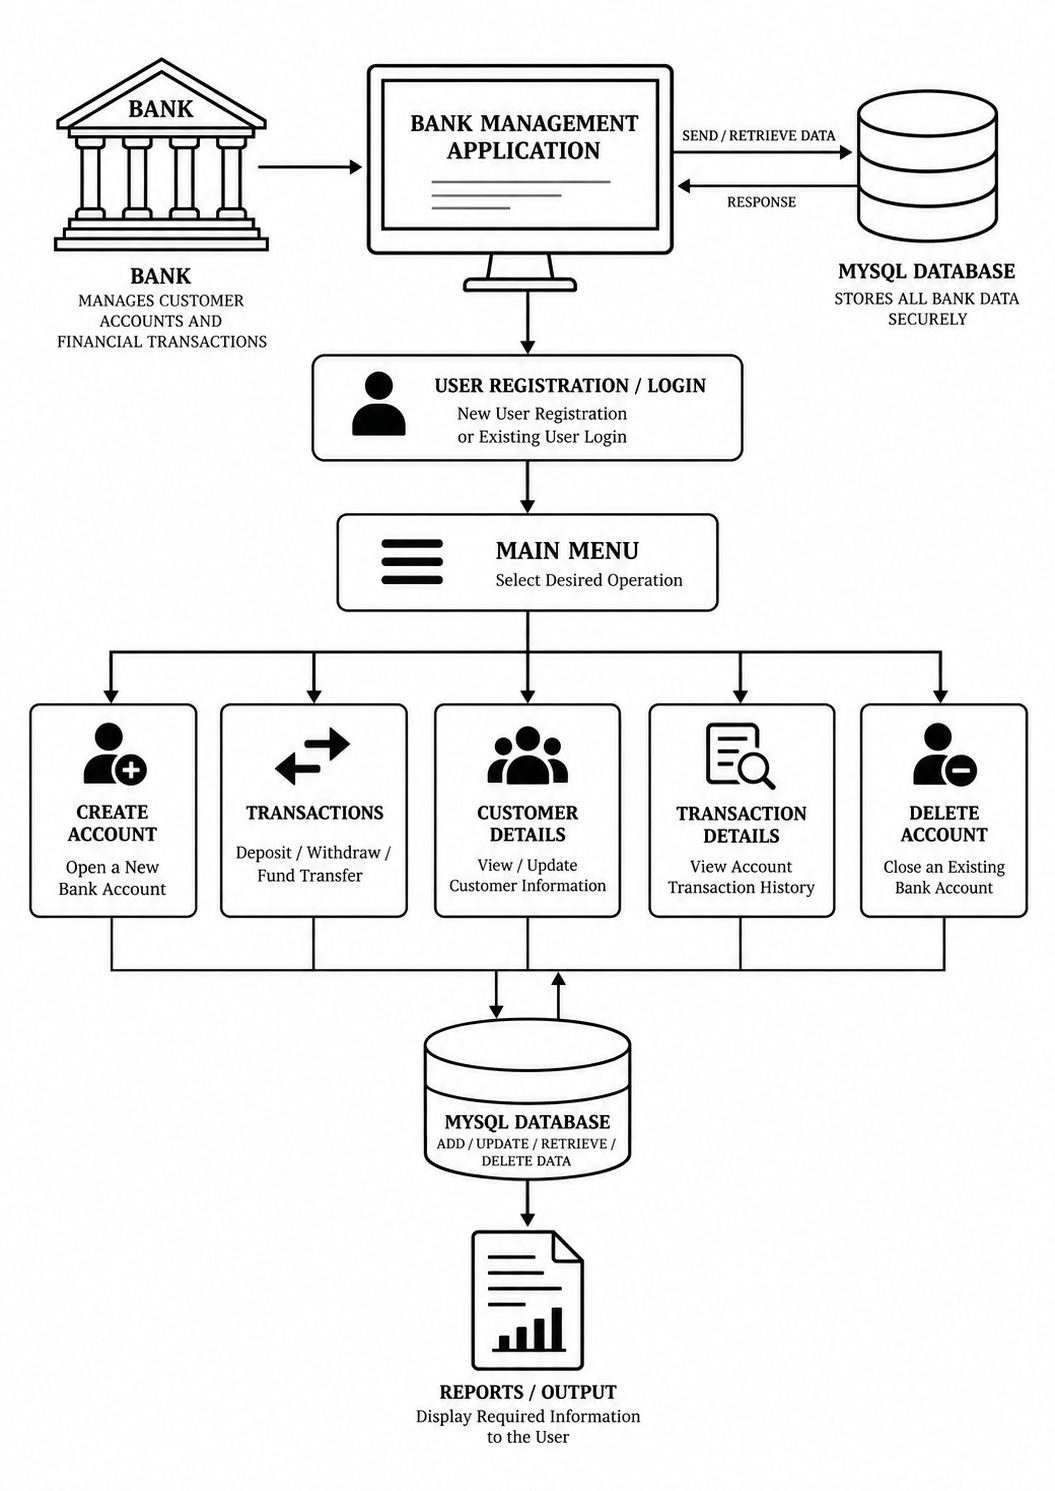
\includegraphics[width=0.66\textwidth]{images/5.png}
    \caption{\textit{Overall Working Process of Bank Management System}}
\end{figure}

\clearpage

% =========================================================================
% PAGE 16: FLOW CHART (Bank Transaction Process)
% =========================================================================
\subsection*{BANK TRANSACTION PROCESS FLOWCHART}
The dedicated flowchart below details the exact decision logic implemented for deposit and withdrawal transactions. It demonstrates account validation, user choice branching, overdraft protection checks, database balance updates, and transaction logging.

\vspace{0.6em}
\begin{figure}[H]
    \centering
    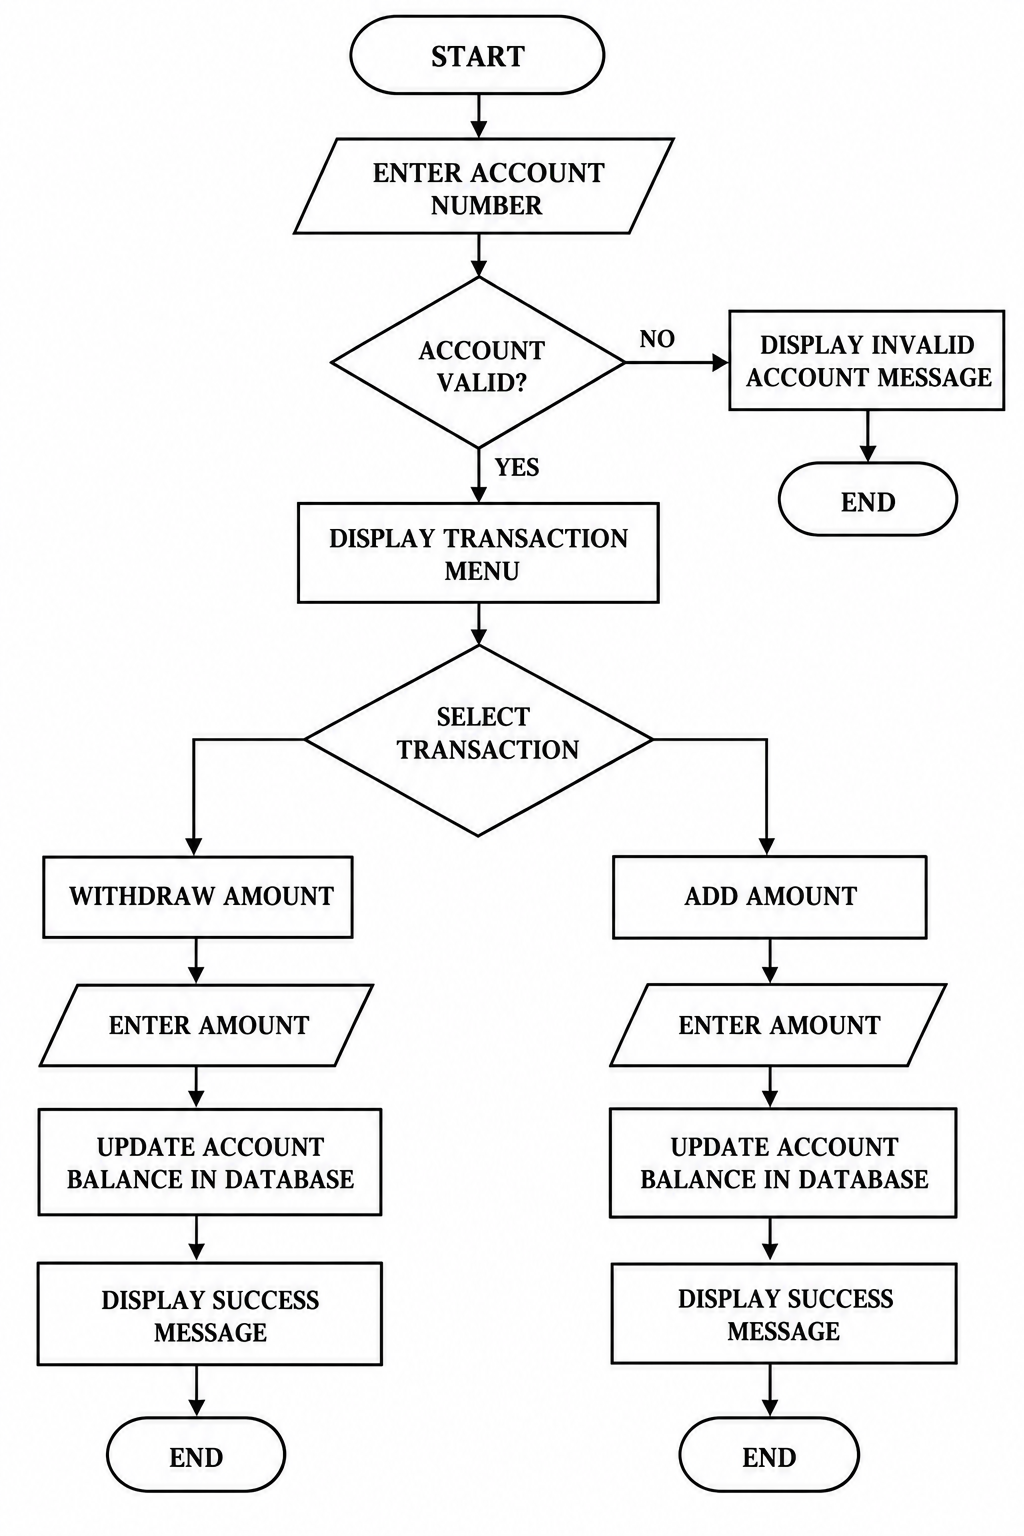
\includegraphics[width=0.60\textwidth]{images/3.png}
    \caption{\textit{Bank Transaction Process Flowchart}}
\end{figure}

\clearpage

% =========================================================================
% PAGE 17: SOURCE CODE (DDL Table Scripts)
% =========================================================================
\phantomsection\hypertarget{sec:sourcecode}{}\label{sec:sourcecode}
\section*{07. SOURCE CODE}
\vspace{0.4em}

\subsection*{1. DATABASE INITIALIZATION SCRIPTS (DDL)}
The following standalone scripts establish the relational database tables in the MySQL \texttt{bank} database:

\vspace{0.4em}
\noindent\textbf{A. Customer Details Table Setup (\texttt{table.py}):}
\begin{lstlisting}[language=Python]
import mysql.connector as sql

conn = sql.connect(host='localhost', user='root', passwd='manager', database='bank')
cur = conn.cursor()

cur.execute('''
    CREATE TABLE IF NOT EXISTS customer_details (
        acct_no INT PRIMARY KEY,
        acct_name VARCHAR(25),
        phone_no BIGINT,
        address VARCHAR(50),
        cr_amt FLOAT
    )
''')
conn.commit()
print("Table 'customer_details' created successfully.")
\end{lstlisting}

\noindent\textbf{B. User Authentication Table Setup (\texttt{user\_table.py}):}
\begin{lstlisting}[language=Python]
import mysql.connector as sql

conn = sql.connect(host='localhost', user='root', passwd='manager', database='bank')
cur = conn.cursor()

cur.execute('''
    CREATE TABLE IF NOT EXISTS user_table (
        username VARCHAR(25) PRIMARY KEY,
        passwrd VARCHAR(25) NOT NULL
    )
''')
conn.commit()
print("Table 'user_table' created successfully.")
\end{lstlisting}

\noindent\textbf{C. Transactions Table Setup (\texttt{transaction\_table.py}):}
\begin{lstlisting}[language=Python]
import mysql.connector as sql

conn = sql.connect(host='localhost', user='root', passwd='manager', database='bank')
cur = conn.cursor()

cur.execute('''
    CREATE TABLE IF NOT EXISTS transactions (
        acct_no INT,
        date DATE,
        withdrawal_amt FLOAT,
        amount_added FLOAT
    )
''')
conn.commit()
print("Table 'transactions' created successfully.")
\end{lstlisting}

\clearpage

% =========================================================================
% PAGE 18: SOURCE CODE (main_bank.py Part 1)
% =========================================================================
\subsection*{2. MAIN SYSTEM ENTRY SCRIPT (\texttt{main\_bank.py} - Part 1)}
The \texttt{main\_bank.py} script acts as the master authentication gatekeeper and security boundary for the Bank Management System. Upon execution, the module initializes runtime dependencies, connects to the local MySQL database instance using host, user, and password parameters, and initializes an operational cursor for transactional communication.

Part 1 implements the application bootstrapper and the operator onboarding sequence. It presents an interactive terminal interface that timestamps system entry using Python's standard \texttt{datetime} module. When Option 1 (Register) is selected, the routine prompts the operator for a new username and a mandatory 4-digit security PIN. It validates the credentials and executes an \texttt{INSERT} query against the \texttt{user\_table} relation, followed by an immediate \texttt{conn.commit()} to ensure persistent ACID storage before launching the main banking menu.

\vspace{0.4em}
\begin{lstlisting}[language=Python]
# main_bank.py - User Authentication and System Gateway
import datetime as dt
import mysql.connector as sql
import menu

# Establishing connection with MySQL server
conn = sql.connect(host='localhost', user='root', passwd='manager', database='bank')
cur = conn.cursor()

print('========================= WELCOME TO STARK BANK =========================')
print(dt.datetime.now())
print('1. REGISTER')
print('2. LOGIN')
print('=========================================================================')
print()

n = int(input('enter your choice = '))
print()

# Option 1: New User Registration
if n == 1:
    name = input('Enter a Username = ')
    passwd = input('Enter a 4 DIGIT Password = ')
    
    # Inserting credentials into user_table
    query = f"INSERT INTO user_table (username, passwrd) VALUES ('{name}', '{passwd}')"
    cur.execute(query)
    conn.commit()
    print()
    print('USER created successfully!')
    print()
    
    # Launch main banking operations menu
    menu.main_menu()
\end{lstlisting}

\clearpage

% =========================================================================
% PAGE 19: SOURCE CODE (main_bank.py Part 2)
% =========================================================================
\subsection*{2. MAIN SYSTEM ENTRY SCRIPT (\texttt{main\_bank.py} - Part 2)}
Continuation of \texttt{main\_bank.py} detailing user authentication and dashboard redirection.

\vspace{0.4em}
\begin{lstlisting}[language=Python]
# Option 2: Existing User Login Authentication
elif n == 2:
    name = input('Enter your Username = ')
    passwd = input('Enter your 4 DIGIT Password = ')
    
    # Verifying credentials against database
    query = f"SELECT * FROM user_table WHERE username = '{name}' AND passwrd = '{passwd}'"
    cur.execute(query)
    
    if cur.fetchone() is None:
        print()
        print('Invalid username or password')
    else:
        print()
        print('Login successful!')
        print()
        # Direct authenticated user to main dashboard
        menu.main_menu()
else:
    print('Invalid choice! Please select 1 or 2.')
\end{lstlisting}

\clearpage

% =========================================================================
% PAGE 20: SOURCE CODE (menu.py Part 1)
% =========================================================================
\subsection*{3. BANKING OPERATIONS MODULE (\texttt{menu.py} - Part 1)}
The \texttt{menu.py} module handles all core banking features. Part 1 covers initialization and Account Creation. Apart from the creation routine itself, this first part establishes the shared database cursor and the master dispatch loop that governs every subsequent operator choice, giving the module a single, predictable entry point.

\vspace{0.4em}
\begin{lstlisting}[language=Python]
# menu.py - Core Banking Operations Dashboard
import datetime as dt
import mysql.connector as sql

conn = sql.connect(host='localhost', user='root', passwd='manager', database='bank')
cur = conn.cursor()

def main_menu():
    while True:
        print()
        print('========================= MAIN MENU =========================')
        print('1. CREATE BANK ACCOUNT')
        print('2. TRANSACTION')
        print('3. CUSTOMER DETAILS')
        print('4. TRANSACTION DETAILS')
        print('5. DELETE ACCOUNT')
        print('6. QUIT')
        print('=============================================================')
        print()

        n = int(input('Enter your CHOICE = '))
        print()

        # Feature 1: Create New Bank Account
        if n == 1:
            acc_no = int(input('Enter your ACCOUNT NUMBER = '))
            acc_name = input('Enter your ACCOUNT NAME = ')
            ph_no = int(input('Enter your PHONE NUMBER = '))
            add = input('Enter your place = ')
            cr_amt = float(input('Enter your credit amount = '))

            query = f"INSERT INTO customer_details VALUES ({acc_no}, '{acc_name}', {ph_no}, '{add}', {cr_amt})"
            cur.execute(query)
            conn.commit()
            print()
            print('Account Created Successfully!!!!!')
\end{lstlisting}

\clearpage

% =========================================================================
% PAGE 21: SOURCE CODE (menu.py Part 2)
% =========================================================================
\subsection*{3. BANKING OPERATIONS MODULE (\texttt{menu.py} - Part 2)}
Continuation of \texttt{menu.py} detailing the financial Transaction Processing engine.

\vspace{0.4em}
\begin{lstlisting}[language=Python]
        # Feature 2: Financial Transactions (Withdrawal & Deposit)
        elif n == 2:
            acct_no = int(input('Enter Your Account Number = '))
            cur.execute(f"SELECT * FROM customer_details WHERE acct_no = {acct_no}")
            data = cur.fetchall()

            if len(data) == 0:
                print()
                print('Account Number Invalid. Please try again.')
            else:
                current_bal = data[0][4]
                print()
                print('1. WITHDRAW AMOUNT')
                print('2. ADD AMOUNT')
                print()
                x = int(input('Enter your CHOICE = '))
                print()
                today_date = dt.date.today()

                # Sub-option 1: Cash Withdrawal with Overdraft Check
                if x == 1:
                    amt = float(input('Enter withdrawal amount = '))
                    if amt > current_bal:
                        print()
                        print('Insufficient Balance!')
                    else:
                        cur.execute(f"UPDATE customer_details SET cr_amt = cr_amt - {amt} WHERE acct_no = {acct_no}")
                        cur.execute(f"INSERT INTO transactions VALUES ({acct_no}, '{today_date}', {amt}, 0)")
                        conn.commit()
                        print()
                        print('Account Updated Successfully!!!!!')

                # Sub-option 2: Cash Deposit
                elif x == 2:
                    amt = float(input('Enter amount to be added = '))
                    cur.execute(f"UPDATE customer_details SET cr_amt = cr_amt + {amt} WHERE acct_no = {acct_no}")
                    cur.execute(f"INSERT INTO transactions VALUES ({acct_no}, '{today_date}', 0, {amt})")
                    conn.commit()
                    print()
                    print('Account Updated Successfully!!!!!')
\end{lstlisting}

\clearpage

% =========================================================================
% PAGE 22: SOURCE CODE (menu.py Part 3)
% =========================================================================
\enlargethispage{\baselineskip}
\subsection*{3. BANKING OPERATIONS MODULE (\texttt{menu.py} - Part 3)}
Continuation of \texttt{menu.py} covering Customer Inquiries, Transaction Logs, Account Deletion, and Quit. These final routines close the operational lifecycle: they present read-only views of customer and transaction data, enforce a confirmed deletion sequence that purges both profile and audit records, and provide a controlled exit path that terminates the session cleanly without leaving the cursor or connection open.

\vspace{0.4em}
\begin{lstlisting}[language=Python, basicstyle=\fontsize{8.5pt}{10.4pt}\selectfont\ttfamily]
        # Feature 3: View Customer Details
        elif n == 3:
            acct_no = int(input('Enter your account number = '))
            print()
            cur.execute(f"SELECT * FROM customer_details WHERE acct_no = {acct_no}")
            data = cur.fetchall()

            if len(data) == 0:
                print('Invalid Account number')
            else:
                for row in data:
                    print('ACCOUNT NO      =', row[0])
                    print('ACCOUNT NAME    =', row[1])
                    print('PHONE NUMBER    =', row[2])
                    print('ADDRESS         =', row[3])
                    print('CURRENT BALANCE =', row[4])
                    print()

        # Feature 4: View Transaction Statements
        elif n == 4:
            acct_no = int(input('Enter your account number = '))
            print()
            cur.execute(f"SELECT * FROM customer_details WHERE acct_no = {acct_no}")
            if cur.fetchone() is None:
                print('Invalid Account number')
            else:
                cur.execute(f"SELECT * FROM transactions WHERE acct_no = {acct_no}")
                data = cur.fetchall()
                if len(data) == 0:
                    print('No transactions found for this account.')
                else:
                    print(f"{'ACC NO':<10} {'DATE':<15} {'WITHDRAWAL':<15} {'DEPOSIT':<15}")
                    print('-' * 55)
                    for row in data:
                        print(f"{row[0]:<10} {str(row[1]):<15} {row[2]:<15} {row[3]:<15}")
                    print()

        # Feature 5: Delete Account
        elif n == 5:
            print('DELETE YOUR ACCOUNT')
            acct_no = int(input('Enter your account number = '))
            cur.execute(f"SELECT * FROM customer_details WHERE acct_no = {acct_no}")
            if cur.fetchone() is None:
                print('Account does not exist!')
            else:
                cur.execute(f"DELETE FROM customer_details WHERE acct_no = {acct_no}")
                cur.execute(f"DELETE FROM transactions WHERE acct_no = {acct_no}")
                conn.commit()
                print()
                print('ACCOUNT DELETED SUCCESSFULLY')

        # Feature 6: Quit Application
        elif n == 6:
            c = input('DO YOU WANT TO EXIT (y/n) = ')
            if c.lower() == 'y':
                print()
                print('THANK YOU PLEASE VISIT AGAIN')
                break

if __name__ == '__main__':
    main_menu()
\end{lstlisting}

\clearpage

% =========================================================================
% PAGE 23: OUTPUT (Welcome & Registration)
% =========================================================================
\phantomsection\hypertarget{sec:output}{}\label{sec:output}
\section*{08. OUTPUT}
\vspace{0.4em}

\subsection*{OUTPUT SCREEN 1: SYSTEM WELCOME \& USER REGISTRATION}
Upon running \texttt{main\_bank.py}, the operator is presented with the Stark Bank header, current timestamp, and entry options. Selecting Option 1 allows the registration of a new operator.

\vspace{0.6em}
\begin{lstlisting}
========================= WELCOME TO STARK BANK =========================
2026-10-26 10:15:32.418291
1. REGISTER
2. LOGIN
=========================================================================

enter your choice = 1

Enter a Username = suryah
Enter a 4 DIGIT Password = 1298

USER created successfully!
\end{lstlisting}

\clearpage

% =========================================================================
% PAGE 24: OUTPUT (Login & Main Menu)
% =========================================================================
\subsection*{OUTPUT SCREEN 2: USER LOGIN \& MAIN MENU DASHBOARD}
Selecting Option 2 prompts the operator for their username and 4-digit security PIN. Upon successful verification against \texttt{user\_table}, the system unlocks the interactive Main Menu.

\vspace{0.6em}
\begin{lstlisting}
========================= WELCOME TO STARK BANK =========================
2026-10-26 10:18:04.120954
1. REGISTER
2. LOGIN
=========================================================================

enter your choice = 2

Enter your Username = suryah
Enter your 4 DIGIT Password = 1298

Login successful!

========================= MAIN MENU =========================
1. CREATE BANK ACCOUNT
2. TRANSACTION
3. CUSTOMER DETAILS
4. TRANSACTION DETAILS
5. DELETE ACCOUNT
6. QUIT
=============================================================

Enter your CHOICE = 
\end{lstlisting}

\clearpage

% =========================================================================
% PAGE 25: OUTPUT (Create Bank Account)
% =========================================================================
\subsection*{OUTPUT SCREEN 3: CREATE BANK ACCOUNT}
Selecting Option 1 initiates account creation. The operator enters customer account number, full name, phone number, location, and initial credit amount.

\vspace{0.6em}
\begin{lstlisting}
========================= MAIN MENU =========================
1. CREATE BANK ACCOUNT
2. TRANSACTION
3. CUSTOMER DETAILS
4. TRANSACTION DETAILS
5. DELETE ACCOUNT
6. QUIT
=============================================================

Enter your CHOICE = 1

Enter your ACCOUNT NUMBER = 1001
Enter your ACCOUNT NAME = Rohan Sharma
Enter your PHONE NUMBER = 9876543210
Enter your place = Delhi
Enter your credit amount = 50000

Account Created Successfully!!!!!
\end{lstlisting}

\clearpage

% =========================================================================
% PAGE 26: OUTPUT (Transaction: Deposit & Withdrawal)
% =========================================================================
\subsection*{OUTPUT SCREEN 4: TRANSACTION PROCESSING}
Selecting Option 2 presents the transaction processing engine. Below are samples of cash deposit and cash withdrawal executions:

\vspace{0.6em}
\begin{lstlisting}
-- TRANSACTION EXECUTION: CASH DEPOSIT --
Enter your CHOICE = 2

Enter Your Account Number = 1001

1. WITHDRAW AMOUNT
2. ADD AMOUNT

Enter your CHOICE = 2

Enter amount to be added = 15000

Account Updated Successfully!!!!!

-- TRANSACTION EXECUTION: CASH WITHDRAWAL --
Enter your CHOICE = 2

Enter Your Account Number = 1001

1. WITHDRAW AMOUNT
2. ADD AMOUNT

Enter your CHOICE = 1

Enter withdrawal amount = 5000

Account Updated Successfully!!!!!
\end{lstlisting}

\clearpage

% =========================================================================
% PAGE 27: OUTPUT (Customer Details & History)
% =========================================================================
\subsection*{OUTPUT SCREEN 5: CUSTOMER DETAILS \& STATEMENT LOG}
Option 3 displays profile information, and Option 4 generates a formatted chronological statement log:

\vspace{0.6em}
\begin{lstlisting}
-- OPTION 3: CUSTOMER DETAILS LOOKUP --
Enter your CHOICE = 3

Enter your account number = 1001

ACCOUNT NO      = 1001
ACCOUNT NAME    = Rohan Sharma
PHONE NUMBER    = 9876543210
ADDRESS         = Delhi
CURRENT BALANCE = 60000.0

-- OPTION 4: TRANSACTION DETAILS AUDIT LOG --
Enter your CHOICE = 4

Enter your account number = 1001

ACC NO     DATE            WITHDRAWAL      DEPOSIT        
-------------------------------------------------------
1001       2026-10-26      0.0             15000.0        
1001       2026-10-26      5000.0          0.0            
\end{lstlisting}

\clearpage

% =========================================================================
% PAGE 28: OUTPUT (Delete Account & Exit)
% =========================================================================
\subsection*{OUTPUT SCREEN 6: DELETE ACCOUNT \& QUIT}
Option 5 terminates customer accounts and removes audit records. Option 6 safely terminates the active session:

\vspace{0.6em}
\begin{lstlisting}
-- OPTION 5: TERMINATE BANK ACCOUNT --
Enter your CHOICE = 5

DELETE YOUR ACCOUNT
Enter your account number = 1001

ACCOUNT DELETED SUCCESSFULLY

-- OPTION 6: SYSTEM EXIT --
========================= MAIN MENU =========================
1. CREATE BANK ACCOUNT
2. TRANSACTION
3. CUSTOMER DETAILS
4. TRANSACTION DETAILS
5. DELETE ACCOUNT
6. QUIT
=============================================================

Enter your CHOICE = 6

DO YOU WANT TO EXIT (y/n) = y

THANK YOU PLEASE VISIT AGAIN
\end{lstlisting}

\clearpage

% =========================================================================
% PAGE 29: TESTING (Overview & Black Box)
% =========================================================================
\phantomsection\hypertarget{sec:testing}{}\label{sec:testing}
\section*{09. TESTING}
\vspace{0.5em}

\subsection*{1. SOFTWARE TESTING OVERVIEW}
Software Testing is an empirical investigation conducted to provide stakeholders with objective information regarding the quality and reliability of the software system under test. It formally verifies that the software satisfies technical requirements and behaves predictably when subjected to invalid, boundary, or malicious inputs.

\vspace{1.2em}
\subsection*{2. BLACK BOX TESTING (SPECIFICATION-BASED TESTING)}
Black Box Testing evaluates functionality without inspecting internal source code logic or algorithmic structures. Test design is driven strictly by external functional specifications.

\vspace{0.4em}
\noindent\textbf{Testing Techniques Applied:}
\begin{itemize}
    \item \textbf{Equivalence Partitioning:} Input domains were categorized into valid partitions (e.g., existing account numbers, positive deposit amounts, 4-digit PINs) and invalid partitions (e.g., negative withdrawals, non-numeric inputs, non-existent accounts).
    \item \textbf{Boundary Value Analysis:} Testing the extreme frontiers of input ranges, such as attempting to withdraw exactly the full account balance ($Balance - Balance = 0$), withdrawing zero currency units, and attempting to withdraw 1 unit beyond available balance.
    \item \textbf{User Scenario Emulation:} Executing standard operational sequences from the perspective of an authorized branch teller to verify usability.
\end{itemize}

\clearpage

% =========================================================================
% PAGE 30: TESTING (White Box Testing)
% =========================================================================
\subsection*{3. WHITE BOX TESTING (STRUCTURAL TESTING)}
White Box Testing examines internal source code logic, control branches, and execution paths. It confirms that internal data structures, relational queries, and loops behave correctly.

\vspace{0.6em}
\noindent\textbf{White Box Testing Methodologies Applied:}
\begin{itemize}
    \item \textbf{Statement Coverage:} Ensuring that every individual line of Python source code and every SQL statement across \texttt{main\_bank.py} and \texttt{menu.py} is executed at least once during test suites.
    \item \textbf{Branch \& Decision Coverage:} Verifying that every conditional decision branch (\texttt{if cur.fetchone() is None}, \texttt{if amt > current\_bal}, \texttt{if len(data) == 0}) is tested under both \texttt{True} and \texttt{False} outcomes.
    \item \textbf{Database Integrity Verification:} Verifying that relational primary key constraints reject duplicate records and that SQL exceptions are caught without abrupt terminal termination.
    \item \textbf{Commit Verification:} Ensuring that atomic commit directives (\texttt{conn.commit()}) are properly placed after every state modification.
\end{itemize}

\clearpage

% =========================================================================
% PAGE 31: TESTING (Test Cases Matrix)
% =========================================================================
\subsection*{4. SYSTEM TEST CASES EXECUTION MATRIX}
The formal test case execution matrix below demonstrates the verification results of the Bank Management System:

\vspace{0.6em}
\begin{center}
\renewcommand{\arraystretch}{1.25}
\small
\begin{tabular}{|c|c|p{4.2cm}|p{2.8cm}|p{2.6cm}|c|}
\hline
\textbf{ID} & \textbf{Mod} & \textbf{Test Description} & \textbf{Test Input} & \textbf{Expected Result} & \textbf{Stat} \\ \hline
TC01 & Auth & Register valid user & suryah, 1298 & User created & PASS \\ \hline
TC02 & Auth & Login with valid PIN & suryah, 1298 & Login successful & PASS \\ \hline
TC03 & Auth & Login with wrong PIN & suryah, 9999 & Invalid credentials & PASS \\ \hline
TC04 & Acct & Create unique account & Acc: 1001, Rs.50000 & Account created & PASS \\ \hline
TC05 & Txn & Deposit valid amount & Acc: 1001, +Rs.15000 & Balance = 65000 & PASS \\ \hline
TC06 & Txn & Withdraw valid amount & Acc: 1001, -Rs.5000 & Balance = 60000 & PASS \\ \hline
TC07 & Txn & Overdraft withdrawal & Acc: 1001, -Rs.90000 & Insufficient Funds & PASS \\ \hline
TC08 & Inq & Lookup valid account & Acc: 1001 & Display details & PASS \\ \hline
TC09 & Inq & Lookup invalid account & Acc: 9999 & Invalid account & PASS \\ \hline
TC10 & Stmt & Check audit logs & Acc: 1001 & Display statements & PASS \\ \hline
TC11 & Del & Delete active account & Acc: 1001 & Account deleted & PASS \\ \hline
\end{tabular}
\end{center}

\clearpage

% =========================================================================
% PAGE 32: HARDWARE & SOFTWARE REQUIREMENTS
% =========================================================================
\phantomsection\hypertarget{sec:hardware}{}\label{sec:hardware}
\section*{10. HARDWARE AND SOFTWARE REQUIREMENTS}
\vspace{0.5em}

\subsection*{1. HARDWARE REQUIREMENTS}
The Bank Management System is optimized for high computational efficiency, running smoothly on modest personal computer configurations:

\vspace{0.6em}
\begin{center}
\renewcommand{\arraystretch}{1.3}
\small
\begin{tabular}{|l|p{5.5cm}|p{6cm}|}
\hline
\textbf{Component} & \textbf{Minimum Requirement} & \textbf{Recommended Specification} \\ \hline
Processor & Intel Pentium / AMD Athlon & Intel Core i3 / AMD Ryzen 3 or higher \\ \hline
RAM & 512 MB RAM & 4 GB RAM or higher \\ \hline
Hard Disk Space & 40 GB SATA HDD & 256 GB SSD (500 MB free for DB) \\ \hline
Display Monitor & 14.1 or 15--17 inch (1024x768) & 1920x1080 Full HD Monitor \\ \hline
Input Devices & Standard Keyboard \& Mouse & Standard QWERTY Keyboard \& Mouse \\ \hline
Printer & Optional (for statements) & Monochrome Laser Printer (B\&W) \\ \hline
\end{tabular}
\end{center}

\vspace{1.5em}
\subsection*{2. SOFTWARE REQUIREMENTS}
\begin{itemize}
    \item \textbf{Operating System:} Microsoft Windows 7 / 8 / 10 / 11 (32-bit or 64-bit).
    \item \textbf{Python Interpreter:} Python 3.12 (or any stable Python 3.7+ release).
    \item \textbf{Database Server:} MySQL Community Server 8.0 (or MySQL 5.7).
    \item \textbf{Python Connector:} \texttt{mysql-connector-python} package.
    \item \textbf{Development Environment:} Python IDLE, VS Code, or Windows PowerShell.
\end{itemize}

\clearpage

% =========================================================================
% PAGE 33: INSTALLATION PROCEDURE
% =========================================================================
\phantomsection\hypertarget{sec:installation}{}\label{sec:installation}
\section*{11. INSTALLATION PROCEDURE}
\vspace{0.5em}

To deploy and execute the Bank Management System in a new environment, follow the step-by-step procedure detailed below:

\vspace{0.6em}
\noindent\textbf{1. Step 1: Install Python Runtime} \\
Download Python 3.12 from \texttt{python.org}. Run the installer and ensure the checkbox \textit{`Add Python.exe to PATH'} is selected. Verify installation by running \texttt{python --version} in the terminal.

\vspace{0.6em}
\noindent\textbf{2. Step 2: Install MySQL Server and Connector} \\
Install MySQL Community Server from \texttt{dev.mysql.com}. Set the root password to \texttt{manager} (or update credentials in the Python source code). Install the MySQL Python connector:
\begin{lstlisting}[language=bash]
pip install mysql-connector-python
\end{lstlisting}

\noindent\textbf{3. Step 3: Create the Relational Database} \\
Open the MySQL Command Line Client, authenticate with your root password, and initialize the project database:
\begin{lstlisting}[language=SQL]
CREATE DATABASE bank;
USE bank;
\end{lstlisting}

\noindent\textbf{4. Step 4: Execute Database Table Schema Scripts} \\
Navigate to the source code folder and execute the three DDL setup scripts sequentially to create the tables:
\begin{lstlisting}[language=bash]
python table.py
python user_table.py
python transaction_table.py
\end{lstlisting}

\noindent\textbf{5. Step 5: Launch the Bank Management Application} \\
Launch the primary system entry file:
\begin{lstlisting}[language=bash]
python main_bank.py
\end{lstlisting}
Follow the interactive prompts to register a user account, authenticate via PIN, and access the main banking dashboard.

\clearpage

% =========================================================================
% PAGE 34: BIBLIOGRAPHY
% =========================================================================
\phantomsection\hypertarget{sec:bibliography}{}\label{sec:bibliography}
\section*{12. BIBLIOGRAPHY}
\vspace{0.8em}

The development, database design, and documentation of this project were guided by the following textbooks, reference materials, and web resources:

\vspace{0.8em}
\subsection*{TEXTBOOKS \& ACADEMIC REFERENCES}
\begin{itemize}
    \item Sumita Arora, \textit{Computer Science with Python --- Textbook for Class XII}, Dhanpat Rai \& Co. Publications.
    \item Preeti Arora, \textit{Computer Science with Python for Class XII}, Sultan Chand Publications.
    \item NCERT, \textit{Computer Science --- Class XII (Python)}, National Council of Educational Research and Training.
    \item Praveen M Jigajinni, \textit{Project Guidance and Reference Material on Bank Management System (BMS)}, Sainik School Amaravathinagar.
\end{itemize}

\vspace{1.5em}
\subsection*{ONLINE DOCUMENTATION \& TECHNICAL REFERENCES}
\begin{itemize}
    \item Python Software Foundation, \textit{Official Python 3.12 Documentation}: \url{https://docs.python.org/3/}
    \item Oracle Corporation, \textit{MySQL 8.0 Reference Manual}: \url{https://dev.mysql.com/doc/refman/8.0/en/}
    \item Oracle Corporation, \textit{MySQL Connector/Python Developer Guide}: \url{https://dev.mysql.com/doc/connector-python/en/}
    \item w3resource, \textit{Python MySQL Database Connectivity Tutorials}: \url{https://www.w3resource.com/python-exercises/mysql/}
    \item GeeksforGeeks, \textit{CBSE Class 12 Computer Science Project Guidelines}: \url{https://www.geeksforgeeks.org/school-learning/}
\end{itemize}

\end{document}
